In this chapter we discuss the implementation of the LSTM models described in Chapter 
\ref{LSTM Theory}. The goal is to use the hydrological data from the datasets
described in Chapter \ref{Data} to predict runoff.
We describe how we preprocess and combine the datasets 
and how the predictions of these models are used to try and gain 
insight into what physical processes our models deem the most important.
\section{Code available as Python package: CamelsML}
Originally a fork of the code in \citet{lstm_second_paper} with a few modifications, 
the machine learning code of this thesis is now implemented to be a fully fledged 
Python package. As the original code it is forked from, it is released under the 
Apache 2.0 license and anyone is therefore free to modify and implement the code 
into their own experiments in the future.
We dub this package CamelsML (CAMELS Machine Learning).


See Appendix \ref{camelsml documentation} for documentation on how to use the python 
package as well as a minimal running example.

\section{Training algorithm}
%The training procedure described here is heavily based on and uses code from 
%\cite{lstm_second_paper}.
\begin{figure}
\centering
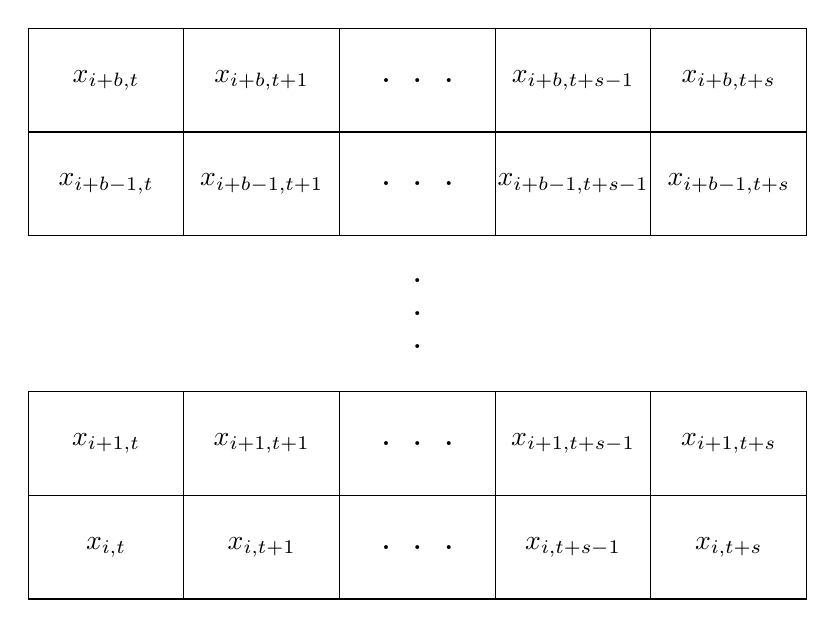
\begin{tikzpicture}[x=0.75pt,y=0.75pt,yscale=-1.25,xscale=1.25]
%uncomment if require: \path (0,300); %set diagram left start at 0, and has height of 300

%Shape: Rectangle [id:dp015989981921256002] 
\draw   (40,200) -- (340,200) -- (340,240) -- (40,240) -- cycle ;
%Shape: Rectangle [id:dp48971481940661865] 
\draw   (40,20) -- (340,20) -- (340,60) -- (40,60) -- cycle ;
%Straight Lines [id:da2960915083454566] 
\draw    (100,20) -- (100,60) ;
%Straight Lines [id:da243954626179525] 
\draw    (160,20) -- (160,60) ;
%Straight Lines [id:da4379878415202513] 
\draw    (220,20) -- (220,60) ;
%Straight Lines [id:da23623272729690736] 
\draw    (280,20) -- (280,60) ;
%Straight Lines [id:da34522789326312586] 
\draw    (100,200) -- (100,240) ;
%Straight Lines [id:da016177459682585327] 
\draw    (220,200) -- (220,240) ;
%Straight Lines [id:da5727133385469978] 
\draw    (280,200) -- (280,240) ;
%Straight Lines [id:da29038977274992184] 
\draw    (160,200) -- (160,240) ;






%Shape: Rectangle [id:dp015989981921256002] 
\draw   (40,160) -- (340,160) -- (340,200) -- (40,200) -- cycle ;
%Shape: Rectangle [id:dp48971481940661865] 
\draw   (40,60) -- (340,60) -- (340,100) -- (40,100) -- cycle ;

%Straight Lines [id:da2960915083454566] 
\draw    (100,60) -- (100,100) ;
%Straight Lines [id:da243954626179525] 
\draw    (160,60) -- (160,100) ;
%Straight Lines [id:da4379878415202513] 
\draw    (220,60) -- (220,100) ;
%Straight Lines [id:da23623272729690736] 
\draw    (280,60) -- (280,100) ;
%Straight Lines [id:da34522789326312586] 
\draw    (100,160) -- (100,200) ;
%Straight Lines [id:da016177459682585327] 
\draw    (220,160) -- (220,200) ;
%Straight Lines [id:da5727133385469978] 
\draw    (280,160) -- (280,200) ;
%Straight Lines [id:da29038977274992184] 
\draw    (160,160) -- (160,200) ;


% Text Node
\draw (190,40) node [anchor=center][inner sep=0.75pt]   [align=left] {{\LARGE . . .}};
% Text Node
\draw (190,220) node [anchor=center][inner sep=0.75pt]   [align=left] {{\LARGE . . .}};
% Text Node
\draw (190,130) node [anchor=center][inner sep=0.75pt]   [align=left] {{\LARGE .}\\{\LARGE .}\\{\LARGE .}};
% Text Node
\draw (70,220) node [anchor=center][inner sep=0.75pt]   [align=left] {$\bm{x}_{i,t}$};
% Text Node
\draw (70,40) node [anchor=center][inner sep=0.75pt]   [align=left] {$\bm{x}_{i+b,t}$};
% Text Node
\draw (130,220) node [anchor=center][inner sep=0.75pt]   [align=left] {$\bm{x}_{i,t+1}$};
% Text Node
\draw (130,40) node [anchor=center][inner sep=0.75pt]   [align=left] {$\bm{x}_{i+b,t+1}$};
% Text Node
\draw (250,40) node [anchor=center][inner sep=0.75pt]   [align=left] {$\bm{x}_{i+b,t+s-1}$};
% Text Node
\draw (250,220) node [anchor=center][inner sep=0.75pt]   [align=left] {$\bm{x}_{i,t+s-1}$};
% Text Node
\draw (310,40) node [anchor=center][inner sep=0.75pt]   [align=left] {$\bm{x}_{i+b,t+s}$};
% Text Node
\draw (310,220) node [anchor=center][inner sep=0.75pt]   [align=left] {$\bm{x}_{i,t+s}$};



\draw (190,80) node [anchor=center][inner sep=0.75pt]   [align=left] {{\LARGE . . .}};
% Text Node
\draw (190,180) node [anchor=center][inner sep=0.75pt]   [align=left] {{\LARGE . . .}};

\draw (70,180) node [anchor=center][inner sep=0.75pt]   [align=left] {$\bm{x}_{i+1,t}$};
% Text Node
\draw (70,80) node [anchor=center][inner sep=0.75pt]   [align=left] {$\bm{x}_{i+b-1,t}$};
% Text Node
\draw (130,180) node [anchor=center][inner sep=0.75pt]   [align=left] {$\bm{x}_{i+1,t+1}$};
% Text Node
\draw (130,80) node [anchor=center][inner sep=0.75pt]   [align=left] {$\bm{x}_{i+b-1,t+1}$};


% Text Node
\draw (250,80) node [anchor=center][inner sep=0.75pt]   [align=left] {$\bm{x}_{i+b-1,t+s-1}$};
% Text Node
\draw (250,180) node [anchor=center][inner sep=0.75pt]   [align=left] {$\bm{x}_{i+1,t+s-1}$};
% Text Node
\draw (310,80) node [anchor=center][inner sep=0.75pt]   [align=left] {$\bm{x}_{i+b-1,t+s}$};
% Text Node
\draw (310,180) node [anchor=center][inner sep=0.75pt]   [align=left] {$\bm{x}_{i+1,t+s}$};
\end{tikzpicture}

    \caption[A mini batch.]{A mini batch. $\bm{x}_{i,t}$ represents the input parameters $\bm{x}$ at time step $t$ for time series $i \in [0, b]$ where $b$ is the batch size. A mini batch consists of $b \times t$ FP32 numbers.}
\label{mini batch}
\end{figure}
The training algorithm excluding mathematical details shown in Chapter \ref{LSTM Theory} 
is shown here:
\begin{enumerate}
    \item Split the training data basin-wise into five parts of equal size.
    \item Repeat the following five times, each time using a different 1/5 of the 
        split data as the validation set: \begin{enumerate}
            \item Initialize LSTM model with random weights and zero biases, except for the bias of the forget gate $\bm{b}_f$, which is initialized as $\bm{b}_f=\bm{5}$.
        \item Split each training time seres into several parts, the length 
            of which is decided by the sequence length variable $s$. A mini batch 
            consists of a batch size $b$ amount of these $s$ long time series. This 
                structure is shown in Figure \ref{mini batch}.
        \item For each mini batch:
        \begin{enumerate}
            \item Use the model to predict the outcomes of each time series in the 
                mini batch. This can be done in parallel.
            \item Use the average loss of all predictions in the mini batch to update 
                the model parameters using ADAM (see (\ref{ADAM.1}-\ref{ADAM.4})).
        \end{enumerate}
        \item Evaluate on the validation set without updating the model parameters.
    \end{enumerate}
\end{enumerate}
We evaluate models using the Nash–Sutcliffe model efficiency coefficient (NSE) \citep{NSE}.
This metric is essentially a hydrological interpretation of the well known $R^2$ score.
It is defined as 
\begin{equation}
    \text{NSE} = 1 - \frac{\sum_{t=0}^T\left( y^t - \hat{y}^t\right)}{\sum_{t=0}^T\left(y^t - \bar{\hat{y}}\right)} \label{NSE}
\end{equation}

Here $T$ is the amount of time steps in a time series, $y^t$ is the observed runoff 
used as the ground truth at time step $t\in[0,T]$, $\tilde{y}^t$ is the predicted runoff at time step $t\in[0,T]$ and $\hat{\tilde{y}}$ is the average predicted runoff.

\citet{lstm_second_paper} argues that using MSE as the cost function is not ideal
for generalized hydrological modelling, as errors on basins with higher absolute 
runoff will contribute more to the total MSE than those with lower runoff. To circumvent 
this they use what they dub the NSE loss function. It is defined as 
\begin{equation}
NSE^*_\text{basin} = \frac{\left| \bm{y}_\text{basin} - \bm{\hat{y}}_\text{basin} 
\right|^2}{\left( \sigma_\text{basin} + \varepsilon \right)^2} \label{NSE loss},
\end{equation}
where $\bm{y}_\text{basin}$ is the observed runoff of a given basin, 
$\bm{\hat{y}}_\text{basin}$ is the predicted runoff of a given basin 
and $\sigma_\text{basin}$ is the standard deviation of a given basin's observed 
runoff. $\varepsilon$ is a very small number included for numerical stability.

As we employ cross validation, we  end up with 5 different models 
for each training run. These models do not necessarily converge to the same model parameters 
as each other, making them potentially quite different from one another. To test the 
actual performance of a model (not just relative to other model configurations) we 
therefore need to train a new model with the same configuration (using the same features, 
hyperparameters, etc.) on the entire, undivided training set and test that model 
on the test set. This test result cannot be used to determine relative performance 
between different model configurations, but it can give an indication of the actual, 
real-world performance of a final selected model. Statistically, this is due to the 
fact that optimizing model configuration using the test set would mean overfitting 
on said test set. See \citet{elemstatlearn} for a more detailed explanation.

For models used to validate transfer learning between CAMELS and CAMELS-GB, we 
cross validate on one dataset and use all five models from the cross validation 
to make ensemble predictions on the validation split of the other dataset. This 
way we can get more robust statistics also in these results, as \citet{lstm_second_paper} 
showed that there often is a non-trivial performance difference between a single
model and a model ensemble. In our case we assume this effect to be even higher 
because of the nature of training and validating on different datasets.

%\section{Model configuration}
%\begin{figure}
%\caption{Our full model configuration using an EA-LSTM \citep{lstm_second_paper}}.
%\end{figure}
\begin{table}
    \centering
    \caption[All LSTM models trained.]{Table containing all models trained in this thesis along with their 
    given labels and configuration. All models are trained with a sequence length of 
    270 days and are initiated with the seed 19970204. 
    The attribute subsets \textbf{\textit{a}}-\textbf{\textit{e}} are shown in Table \ref{attribute table}.}
    \begin{tabular}{llll}
    \toprule
    Label & attribute subset & batch size & dropout rate\\
    \midrule
    GB$_\text{ea-lstm, all}$ & a &  1536 \\
    GB$_\text{lstm, all}$ & a & 1024 \\
    GB$_\text{ea-lstm, chosen}$ & b & 1152 \\
    GB$_\text{lstm, chosen}$ & b & 1280 \\
    GB$_\text{none}$ & n/a & 1280 \\
    US$_\text{Kratzert}$  & c & 1024 \\
    US$_\text{none}$  & n/a & 2048 \\
    Mixed$_\text{ea-lstm}$ & d & 1024 \\
    Mixed$_\text{lstm}$ & d & 1024 \\
    Mixed$_\text{none}$ & n/a & 1024 \\
    Transfer$_\text{GB, ea-lstm}$ & d  & 1024 \\
    Transfer$_\text{GB, lstm}$ & d  & 4096 \\
    Transfer$_\text{GB, none}$ & n/a & 1024 \\
    Transfer$_\text{US, ea-lstm}$ & d & 4096 \\
    Transfer$_\text{US, lstm}$  & d & 4096 \\ 
    Transfer$_\text{US, none}$  & n/a & 4096 \\
    Transfer$_\text{US, ea-lstm 2}$ & e & 2048 \\

\end{tabular}

    \label{all models}
\end{table}
\begin{landscape}
\begin{table}
    \centering
    \caption[All basin attribute subsets.]{Table containing all basin attribute subsets. Subset \textbf{\textit{e}} is equal 
    to subset \textbf{\textit{d}} but without organic\_perc and gvf\_max.}
    \begin{tabular}{ll|lllll}
\hline 
\multicolumn {2}{c}{a}  &  b & c & d & e & f \\
\hline
num\_reservoir & reservoir\_cap & area \\
 dwood\_perc & ewood\_perc & elev\_10\\
 grass\_perc & shrub\_perc & elev\_50\\
 crop\_perc urban\_perc & elev\_90 \\
 inwater\_perc &bares\_perc & dwood\_perc \\
 p\_mean & pet\_mean & ewood\_perc \\
 aridity & p\_seasonality & grass\_perc \\
 frac\_snow & high\_prec\_freq & shrub\_perc \\
 high\_prec\_dur & low\_prec\_freq & crop\_perc \\
 low\_prec\_dur & inter\_high\_perc & urban\_perc \\
 inter\_mod\_perc & inter\_low\_perc & inwater\_perc \\
 frac\_high\_perc & frac\_mod\_perc & bares\_perc \\
 frac\_low\_perc & no\_gw\_perc & sand\_perc \\
 low\_nsig\_perc & nsig\_low\_perc & silt\_perc \\
 gauge\_lat & gauge\_lon & clay\_perc \\
 gauge\_easting & gauge\_northing & organic\_perc \\
 gauge\_elev & area & bulkdens \\
 elev\_min & elev\_10 & tawc \\
 elev\_50 & elev\_90 & porosity\_cosby \\
 elev\_max & sand\_perc & porosity\_hypres \\
 silt\_perc & clay\_perc & conductivity\_cosby \\
 organic\_perc & bulkdens & conductivity\_hypres \\
 tawc & porosity\_cosby & root\_depth \\
 porosity\_hypres & conductivity\_cosby & soil\_depth\_pelletier \\
 conductivity\_hypres & root\_depth & inter\_high\_perc \\
 soil\_depth\_pelletier & & inter\_high\_perc \\
& & inter\_mod\_perc \\
& & inter\_low\_perc \\
& & frac\_high\_perc \\
& & frac\_mod\_perc \\
& & frac\_low\_perc \\
& & no\_gw\_perc \\
& & low\_nsig\_perc \\
& & nsig\_low\_perc \\
\end{tabular}

    \label{attribute table}
\end{table}
\end{landscape}

Table \ref{all models} shows all trained models from which results are presented in this 
thesis. The largest differences between these models are often which basin attributes 
are included in the training process. Other relevant hyperparameters are set equal 
to the model configuration in \citet{lstm_second_paper}. For CAMELS-GB the dates included 
in the training process are time daily time steps from October 10th 1971 to September 
30th 2015.
For CAMELS the dates used are January 1st 1980 to December 31st 2008.
One should be able to reproduce the results 
of this work using CamelsML Table \ref{attribute transfer}, \ref{all models} and \ref{attribute table}. 
Doing exhaustive validation to decide which subset of attributes to use is not 
feasible with the amount of attributes present in the data of interest. What we instead 
do to end up with the subsets in Table \ref{attribute table} is a mix of a priori 
knowledge and validation: First we manually check which attributes to include based 
on perceived importance in accordance to known physical processes related to rainfall-runoff 
modelling. After training a model on a subset, we evaluate it using cross validation 
as mentioned earlier in this chapter. To give further context for the chosen subsets 
\textbf{\textit{a}}-\textbf{\textit{e}} we present this short summary:
\begin{itemize}
    \item \textbf{\textit{a}}: This is a subset using all numerical static attributes in CAMELS-GB 
        \citep{CAMELS_GB} that are not derived from the outcome (runoff). 
    \item \textbf{\textit{b}}: This is a smaller subset of the static attributes contained in CAMELS-GB. 
        This subset was created with emphasis on perceived importance with respect 
        to known physical processes. As many process-driven models (see Section \ref{VIC} and \ref{NWM}) have a high 
        emphasis on radiation (from vegetation), soil types and land cover we have 
        included all attributes related to soil, water content, vegetation and general land cover. 
        The geographical layout of a basin is also of interest and elevation attributes 
        are therefore included. The inclusion of the feature p\_mean (mean precipitation)
        is however not 
        physically motivated and merely stems from the fact that it was recognized 
        as one of the most important features in \citet{lstm_second_paper}'s analysis 
        using LSTMs on CAMELS \citep{CAMELS_US}. Mean precipitation should in 
        theory be information already given in the precipitation time series, but 
        our models do not have access to the entire precipitation time series while 
        training because of the limited sequence length. 
    \item \textbf{\textit{c}}: This attribute selection is taken from \cite{lstm_third_paper} and 
        is used to reproduce the results of said paper with a different cross validation 
        setup to better fit with the rest of our analysis. \cite{lstm_third_paper} 
        used 12-fold cross validation while we use the more commonly employed 
        5-fold cross validation. 
    \item \textbf{\textit{d}}: This is an attribute selection used for training models on both 
        CAMELS and CAMELS-GB at the same time in addition to transfer learning. 
        The attribute names stated in Table \ref{attribute table} are based on the 
        attribute names in CAMELS-GB. CAMELS and CAMELS-GB have different attributes 
        and different names for the same attributes. Which attributes we deem to 
        be equivalent are shown in Table \ref{attribute transfer}.
    \item \textbf{\textit{e}}: The attributes organic\_perc and gvf\_max are excluded in this subset, 
        otherwise it is identical to subset e. We exclude these two features because 
        of uncertainty of whether our synthetic attribute creation works.
\end{itemize}

\section{Preprocessing and combining datasets}
In statistical models it is important to have all inputs and outputs in unit-less 
form. A common way to achieve this is to normalize each input feature and outcome 
feature \citep{elemstatlearn}. 
We split the data basin-wise into train (75\%) and test (25\%) sets. 
Five-fold cross validation is used on the training set to evaluate model performance.
For each fold in the cross validation run, the data is normalized based on the current 
training set, excluding the chosen validation set in each cross validation iteration.
Mathematically this can be written as 
\begin{equation}
    \bm{a}_\text{norm} = \frac{\bm{a} - \bar{\bm{a}}_\text{train}}{\sigma_{\bm{a}_\text{train}}}. \label{normalization}
\end{equation}
Here $\bm{a}$ represents any variable, input or output, $\hat{\bm{a}}_\text{train}$ is 
the average of said variable in the train set and $\sigma_{\bm{a}_\text{train}}$ is 
the standard deviation of said variable in the train set. If $\bm{a}$ is a time series, 
the averaging is still done for all time steps in all basins in the training set, 
not individually per basin. This normalization is implemented in CamelsML by saving 
the standard deviations and averages of each feature in the training set to the disk 
and is implemented by us. \citet{lstm_third_paper} has likely also implemented this 
in a different way, but this code is not used here.

\begin{table}
    %\begin{adjustbox}{width=\textwidth}
    \centering
        \caption[Common attributes and timeseries CAMELS and CAMELS-GB.]{Timeseries and attributes in CAMELS and CAMELS-GB that we treat as 
    equivalent. The names are taken directly from \citet{CAMELS_US} and \citet{CAMELS_GB}.}
    \begin{tabular}{l|l}
\toprule
Camels-US &     Camels-GB \\
\midrule
time series: & \\
\midrule
prcp$($mm$/$day$)$ $[$mm$/$day$]$ & precipitation [mm/day] \\
    $\frac{\text{tmax} + \text{tmin}}{2}$ [K] & temperature [K]\\
    srad(W/m2) [W$/$m$^2$] & shortwave\_rad [W$/$m$^2$] \\
\midrule
    attributes: & \\
\midrule
elev\_mean [m]  & elev\_mean [m] \\
area\_gages2 [km$^2$] & area [km$^2$] \\
p\_mean [mm/day] & p\_mean [mm/day] \\
    pet\_mean [mm/day] & pet\_mean [mm/day] \\
p\_seasonility & p\_seasonality \\
frac\_snow & frac\_snow \\
    high\_prec\_freq [days / yr] & high\_prec\_freq [days / yr] \\
    high\_prec\_dur [days] & high\_pref\_dur [days]  \\
    low\_prec\_freq [days / yr] & low\_prec\_freq [days / yr] \\
    low\_prec\_dur [days] & low\_prec\_dur [days] \\
aridity & aridity \\
forest\_frac & dwood\_frac + ewood\_frac \\ 
root\_depth\_50 [m] & root\_depth\_50 [m] \\
soil\_depth\_pelletier [m] & soil\_depth\_pelletier [m] \\
soil\_porosity & porosity\_cosby \\
soil\_conductivity [cm/h] & conductivity\_cosby [cm/h] \\
sand\_frac & sand\_perc  / 100 \\
silt\_frac & silt\_perc / 100 \\ 
clay\_frac & clay\_perc  / 100 \\ 
organic\_frac & organic\_perc / 100 \\
    gvf\_max & $1 -\frac{\text{urban\_perc}+\text{inwater\_perc}}{100} $ \\
\bottomrule
\end{tabular}


    %\end{adjustbox}
    \label{attribute transfer}
\end{table}
When using a combination of CAMELS and CAMELS-GB we are limited in both which 
time series and which basin attributes we can use.
As seen in Chapter \ref{data} there are only two overlapping time series: precipitation 
and shortwave radiation. CAMELS-GB only has 
average daily temperature, while CAMELS has both minimum and maximum temperature 
per day. To include temperature as a feature we therefore make the assumption that 
\begin{equation}
    \bar{t}_\text{daily} \approx \frac{t_\text{min, daily} + t_\text{max, daily}}{2} \label{average temp}
\end{equation}
where $\hat{t}_\text{daily}$ is the day-averaged temperature, $t_\text{min, daily}$ is 
the day-minimum temperature and $t_\text{max, daily}$ is the day-maximum temperature.
The assumption in (\ref{average temp}) only holds when the daily temperature maxima 
and minima vary symmetrically around an equilibrium.
Most of the basin attributes we include in the combined dataset have natural equivalents 
in both datasets, but there are two exceptions. We get an equivalent of the attribute 
forest\_frac in CAMELS in CAMELS-GB by assuming that
\begin{equation}
    \text{forest\_frac}_\text{GB} \approx \text{dwood\_frac} + \text{ewood\_frac}. \label{forest gb}
\end{equation}
As described in \citet{CAMELS_GB} dwood\_perc is the percentage of deciduous woodland 
and ewood\_frac is the percentage of evergreen woodland.
Our reasoning for (\ref{forest gb}) is that dwood\_frac and ewood\_frac are the only 
forest attributes in CAMELS-GB and it should therefore be safe to assume that adding 
these together yields the total percentage of wood cover.

For the CAMELS attribute gvf\_max we make a less safe assumption. \citet{CAMELS_US} 
describes this attribute as "maximum monthly mean of the green vegetation fraction". 
It could then follow that the if we subtract all land covers without vegetation 
we end up with something similar. In CAMELS-GB the two land covers not covered in 
vegetation are urban\_perc (percentage of suburban or urban land) and inwater\_perc 
(the percentage covered by inland water). This yields
\begin{equation}
    \text{gvf\_max}_\text{GB} \approx 1 - \frac{\text{urban\_perc} + \text{inwater\_perc}}{100}. \label{gvf gb}
\end{equation}
A full overview of attributes deemed equivalent in CAMELS and CAMELS-GB is shown in 
Table \ref{attribute transfer}.

\begin{figure}
    \centering
    \includegraphics{feature_comparison_mixed/big_boxplot_mixed_validation.pdf}
    \caption[Attribute boxplots CAMELS and CAMELS-GB.]{Boxplots of the basin attributes in CAMELS and CAMELS-GB compared. 
    In each subplot CAMELS-GB is on the left, CAMELS is on the right. The basins included in this 
    figure are the basins contained in the full training set used by all models 
    in this analysis. The orange line indicated the median, the green dashed line indicates the average. }
    \label{attribute comparison}
\end{figure}
Figure \ref{attribute comparison} shows boxplots of the training data of all attributes 
in attribute subset \textbf{\textit{d}} (see Table 
\ref{attribute table}) for both CAMELS and CAMELS-GB. In each subplot CAMELS-GB is 
on the left and CAMELS is on the right. We see that most attributes have higher 
variance in CAMELS than in CAMELS-GB. Exceptions to this are organic\_perc and gvf\_max. 
We therefore include transfer learning models both with and without these two features. 
This also implies that the assumption made in (\ref{gvf gb}) may not be of use.
%\subsection{Feature selection}
\section{Basin attribute ranking}
%\subsubsection{Permutation test}
\label{Feature selection}
One of the criticisms of machine learning models
is that they are not easily interpretable. This 
is especially true if one wants to train a model 
on a dataset with an overwhelming amount of 
features. 
 To interpret our models we implement a way to determine feature importance. There 
are many algorithms to determine feature importance, we choose to use the permutation 
test for its simplicity and ability to be used on any type of trained model.
Given a feature $j$, the permutation importance 
$i_j$ is equal to 
\begin{equation}
i_j = s - \frac{1}{K} \sum_{k=1}^K s_{k,j}\quad 
\label{Permutation equation}
\end{equation}
\citep{permutation,breiman2001random}.
Here $K$ denotes how many permutations we average over for each feature, $s$ is
the model's score on the original data and $s_{k,j}$ is the score of permutation 
number $k$ of the feature $j$. In essence (\ref{Permutation equation}) describes 
how much the performance of a model varies when scrambling the information 
contained in a feature, therefore explaining the importance of the feature 
according to the current model. It is then important to remember that this is not 
the true importance of the feature, only the importance the model thinks the feature 
has. The scoring method $s$ can be any model scoring statistic, often the $R^2$. 
score for regression.
In our case we employ (\ref{NSE}) as the scoring metric and we only consider basins 
with an NSE of at least 0.5, as an NSE / R$^2$ score indicates that a model's 
prediction is at least as good as always predicting the average outcome.

A major problem for this method is that (\ref{Permutation equation}) could give 
unrealistically low significance to features that are highly correlated to other 
features. In this case the feature may very well be important, but the information 
contained in it is also contained in one or more other correlated features, meaning 
the model doesn't lose as much information as one may think. Essentially the rule 
of thumb is that the feature importance is the feature's importance as learned by 
the model, not the actual real world importance. 

To validate that this method is implemented correctly and gives meaningful results 
in our case we train a model on CAMELS-GB that in addition to the attributes in 
attribute subset a of Table \ref{attribute table} has access to attributes directly 
derived from the runoff. This model cannot be used for anything but to validate 
the permutation test as it having access to parts of the outcome as an input 
compromises it's ability to do predictions on ungauged basins.  The attributes in 
question are stated in Table 2 in \citet{CAMELS_GB} under the "Hydrologic signatures" 
class. One of them is for instance q\_mean which is the mean daily discharge (runoff).
\section{Hardware}
The models are run on three different hardware configurations. The important difference 
between these hardware configurations is the amount of available VRAM. As LSTM models 
are recurrent neural networks they are not as parallelizable as other machine learning 
models (see Section \ref{RNN Theory} and \ref{LSTM Theory}). This means that the only way for us to fully exploit 
an increase in VRAM is to parallelize data-wise. To do this we increase the batch size.
The three hardware configurations are listed as follows \footnote{Note that we only 
state the used graphics card as this is the only important difference, we run no 
calculations on processors and do not use a significant amount of ordinary RAM.}:
\begin{enumerate}
    \item Nvidia\textregistered  GTX\texttrademark  980 ti: This has 6 GB of VRAM. We find a batch size of $b\in{1024, 1536}$ 
     depending on the model size to be a sweet spot here.
    \item Nvidia\textregistered   GTX\texttrademark  1660 ti: This GPU is similar to the GTX 980 ti and has the 
        same amount of VRAM. Therefore the same batch sizes apply here too.
    \item Nvidia\textregistered   Tesla\texttrademark  V100 (Provided by Simula's eX3 cluster): This has 32 GB of VRAM. 
        We find a batch size of $b\in[2048,4096]$ depending on the model size
        to be a sweet spot. Anything more leads to a downgrade in speed because 
        of limitations in transferring data from the storage device to the GPU. 
        This is still not ideal and leads to an approximate 30\% utilization of the 
        GPU.
\end{enumerate}
We acknowledge that the inconsistent use of batch sizes across models may somewhat 
impact the model performance, as previously stated in Section \ref{GD Theory}.
However, as long as the amount of mini batches is sufficiently smaller than the number of data points we 
still get an acceptable amount of stochasticity in the training process. As an increase 
in batch size is often directly correlated to the speed of training, the batch size usually set as high as the hardware supports. This is in most cases fine as long 
as the total size of training data is much larger than the available RAM (if training on CPU) or VRAM (if training on GPU).
Still, in an ideal situation we would use the same hardware for all training runs.
%but in this case we are limited by queue times on Simula's eX3 cluster in addition 
%to the as of Q4 2020 $\rightarrow$ Q2 2021 silicon shortage making the acquisition of 
%new graphics cards next to impossible \citep{GPUShortage}.
